\documentclass[Orbiter User Manual.tex]{subfiles}
\begin{document}

\section{Cockpit views}
\label{sec:cockpit_views}
Orbiter can represent a spacecraft cockpit in different ways:

\begin{itemize}
\item with a generic "glass cockpit" view, consisting of two MFD displays, the HUD and a few essential controls. The glass cockpit mode is available for all spacecraft and can be useful for an unobstructed view of the surroundings.
\item With one or several spacecraft-specific 2-D instrument panels.
\item With a virtual 3-D representation of the cockpit.
\end{itemize}

\noindent
The modes can be cycled with \keystroke{F8}. Not all spacecraft may support all cockpit modes, but the glass cockpit is always available. In all three modes, instruments can be operated with the mouse.

\begin{figure}[H]
  \centering
  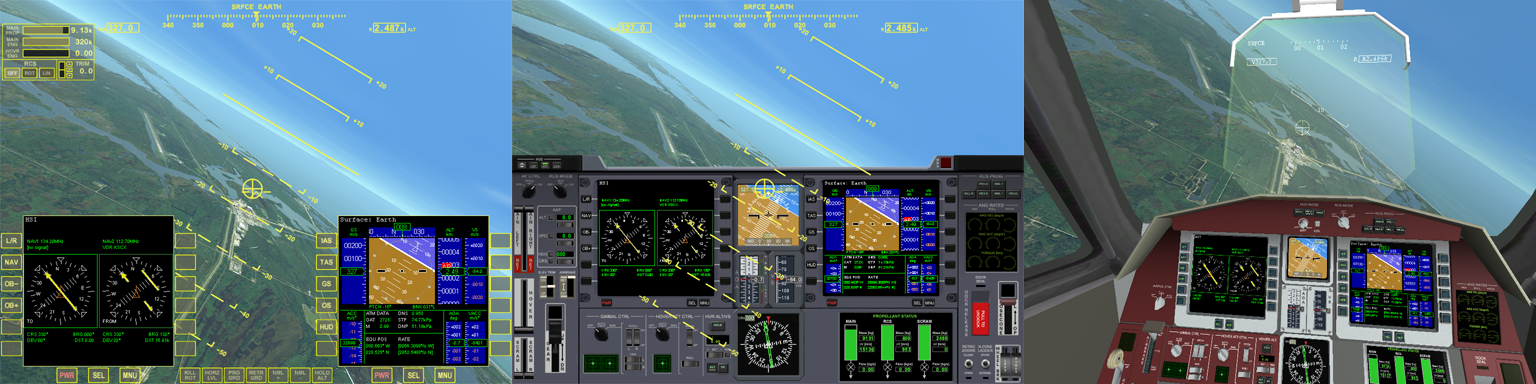
\includegraphics[width=0.99\hsize]{cockpit_comp.png}
  \caption{Comparison of glass cockpit, 2-D panel and virtual cockpit views for the Delta-glider.}
\end{figure}


\subsection{Glass cockpit}
\label{ssec:glass_cockpit}
The generic glass cockpit mode represents a head-up display (HUD) that projects various avionics data directly onto the pilot's forward view. This mode is available for all spacecraft types and provides access to some essential avionics data, MFD instruments and basic flight controls sufficient for basic vessel control in most situations. It does not provide spacecraft-specific instruments and interfaces. For access to these, the 2-D panel or 3-D virtual cockpit view should be used.

\begin{figure}[H]
  \centering
  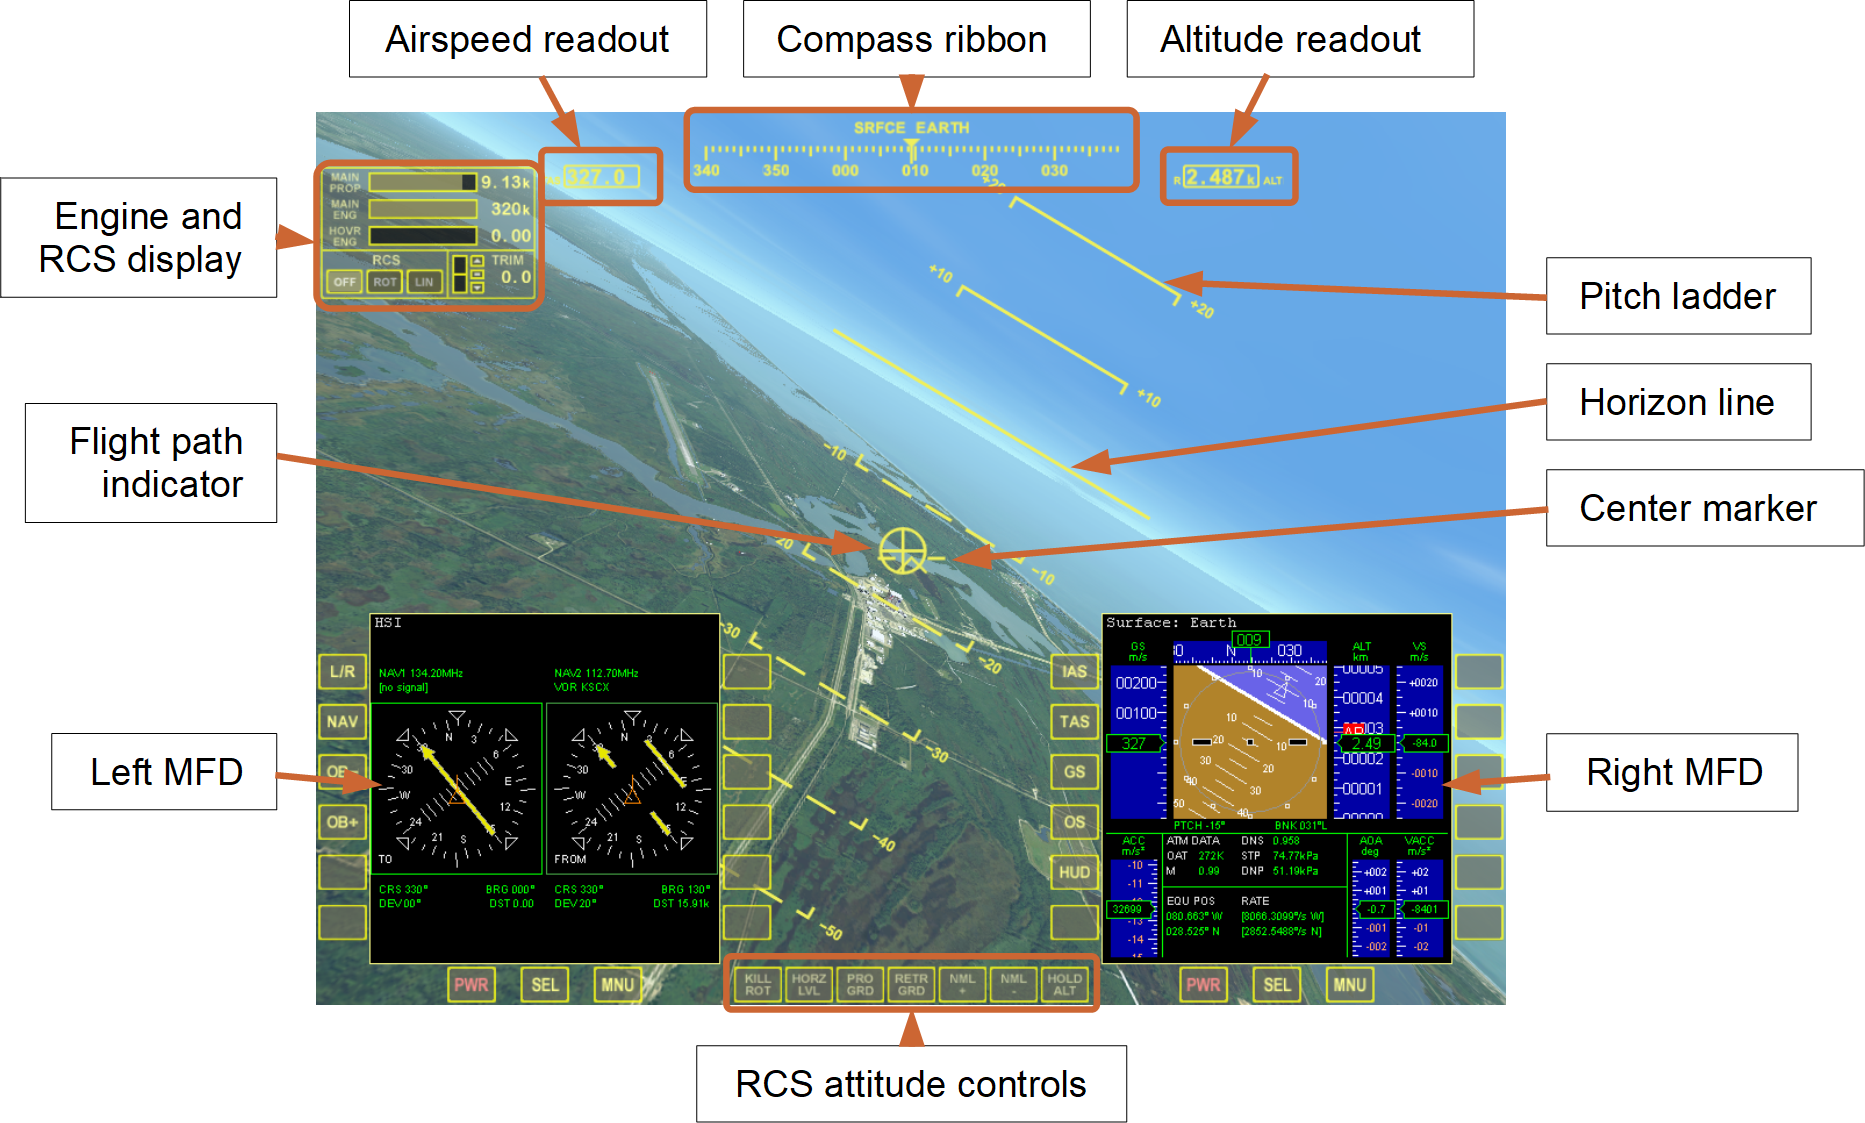
\includegraphics[width=0.99\hsize]{cockpit_glass.png}
\end{figure}

\noindent
The camera direction can be changed by right-clicking and dragging the mouse. However some HUD elements like the centre marker and pitch ladder are only displayed when the camera is looking straight ahead. To return to the default forward view, press \Home$_{Cur}$.\\
\\
\textbf{Engine and RCS display}\\
This display block in the top left corner of the glass cockpit shows the current engine status and provides controls for RCS mode and pitch trim.

\begin{itemize}
\item \textbf{Fuel status:} Shows the propellant remaining in the main fuel tank. The numeric readout is fuel mass [kg]. Note that the vessel may have additional fuel tanks not shown in the generic glass cockpit view. Use vessel-specific 2-D or 3-D cockpit view for detailed fuel information.
\item \textbf{Main engine:} The main engine bar shows the current main/retro engine thrust as a fraction of max. thrust. Green indicates main thrusters active, red indicates retro thrusters active (where applicable). The numerical readout is the thrust force generated [N]. 
\item \textbf{Hover engine:} If the vessel is fitted with hover engines, this bar shows the current hover engine thrust as a fraction of main thrust. Hover engines generate vertical (up) thrust to assist in vertical take-offs and landings, in particular on planetary bodies without atmospheres. The numerical readout is the thrust force generated [N].
\item \textbf{RCS mode indicators:} Shows the current setting of the RCS (reaction control system). The RCS can be OFF, ROT (rotational mode) or LIN (linear mode). See section \ref{ssec:control_att} for details on attitude control. The indicator buttons can be clicked with the mouse to set the mode.
\item \textbf{Trim control:} The vertical bar shows the current pitch trim settings for the vessel's aerodynamic control surfaces, if present. The trim setting can be adjusted with the three buttons next to the bar. (top button: nose up, bottom button: nose down, centre button: trim neutral).

\end{itemize}


\begin{figure}[H]
  \centering
  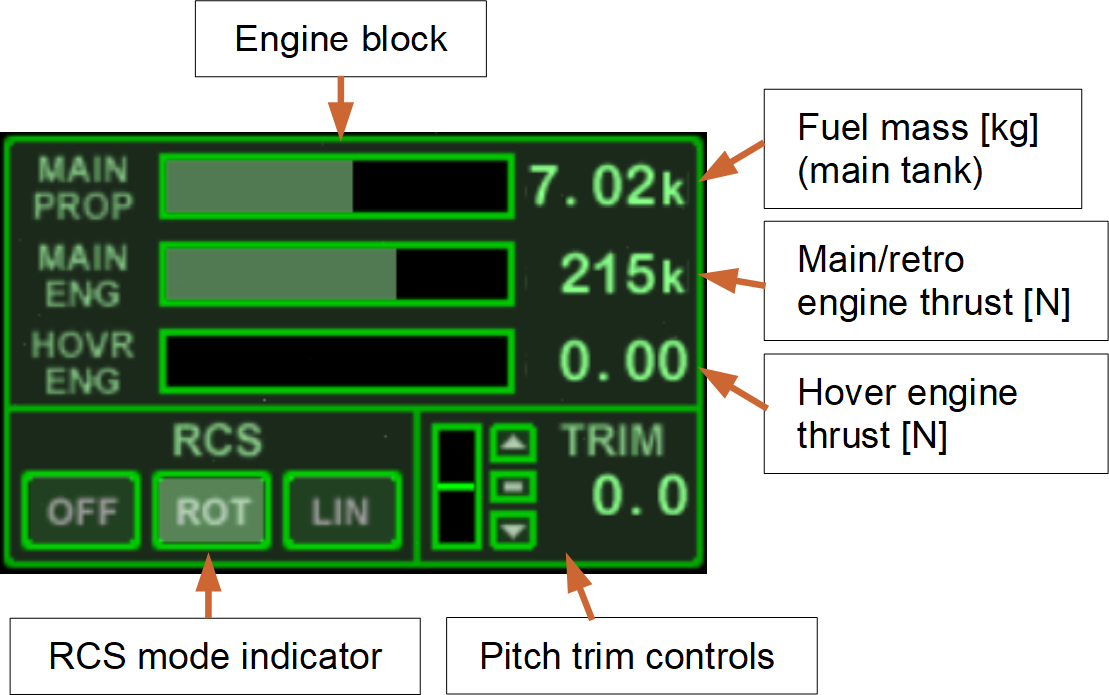
\includegraphics[width=0.5\hsize]{cockpit_glass_disp.png}
  \caption{Glass cockpit engine and RCS display block}
\end{figure}

\noindent
\\
\textbf{RCS attitude controls}\\
The seven buttons along the bottom centre of the glass cockpit screen provide an interface to some basic attitude control modes. Clicking a button activates or deactivates the corresponding mode. The active mode is indicated by a highlighted button. Activating a mode will deactivate any conflicting modes (except HOLDALT which is independent of other modes). An active mode engages the RCS thrusters to rotate and hold the vessel in a specific surface or orbit-relative attitude (with the exception of the \textit{Hold altitude} mode which addresses the hover thrusters if available).

\begin{figure}[H]
  \centering
  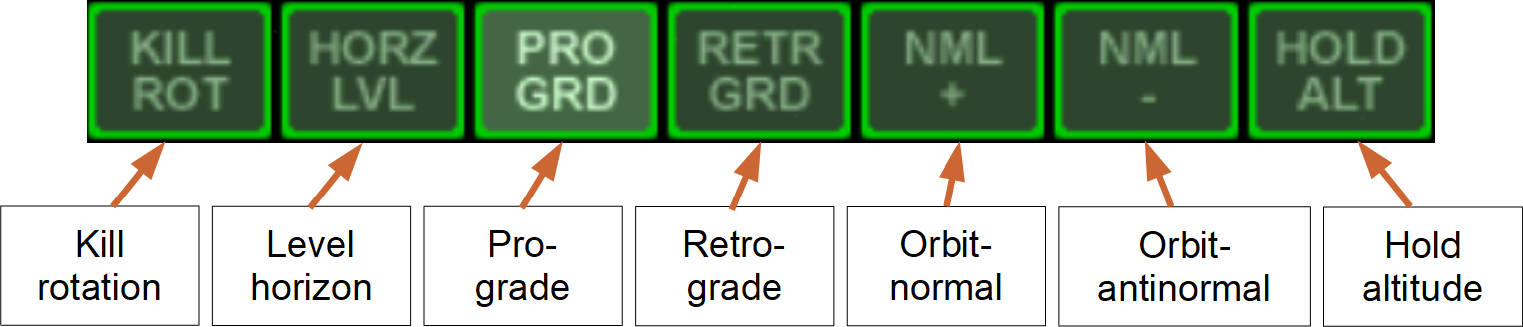
\includegraphics[width=0.75\hsize]{cockpit_glass_mode.png}
\end{figure}

%\begin{table}[H]
	%\centering
	\begin{longtable}{ |p{0.15\textwidth}|p{0.15\textwidth}|p{0.6\textwidth}| }
	\hline\rule{0pt}{2ex}
	\textbf{Mode} & \textbf{Shortcut} & \textbf{Action}\\
	\hline\rule{0pt}{2ex}
	KILLROT & \keystroke{5}$_{Num}$ & Cancel any vessel rotation (auto-terminates)\\
	\hline\rule{0pt}{2ex}
	HORZLVL & \keystroke{L} & Keep vessel level with local horizon\\
	\hline\rule{0pt}{2ex}
	PROGRD & \keystroke{[} & Prograde (turn vessel to orbital velocity vector)\\
	\hline\rule{0pt}{2ex}
	RETRGRD & \keystroke{]} & Retrograde (turn vessel to negative orbital velocity vector)\\
	\hline\rule{0pt}{2ex}
	NML+ & \keystroke{;} & Orbit-normal (turn vessel normal to orbital plane)\\
	\hline\rule{0pt}{2ex}
	NML- & \keystroke{'} & Orbit-antinormal (turn vessel to negative normal of orbit plane)\\
	\hline\rule{0pt}{2ex}
	HOLDALT & \keystroke{A} & Hold altitude (hover function)\\
	\hline
	\end{longtable}
%\end{table}

\noindent
The PROGRD and RETRGRD modes turn the vessel to align with the orbital velocity vector or in the opposite direction. These modes are important for in-plane manoeuvres (e.g. increasing/decreasing the orbit radius). The NML+ and NML- modes turn and hold the vessel perpendicular to the orbital plane. These modes are important for plane change manoeuvres. The HORZLVL mode rotates the vessel to be level with the local horizon. KILLROT engages the RCS system to cancel out any rotation and automatically switches off once the vessel's angular velocity is zero.

\begin{figure}[H]
  \centering
  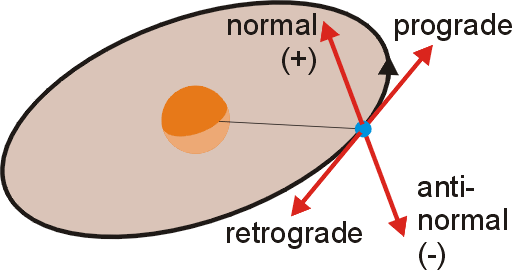
\includegraphics[width=0.5\hsize]{orbit_dir.png}
\end{figure}

\noindent
The HOLDALT mode engages the vessel's hover thrusters (if available) to maintain the current altitude. This mode works best with a level flight attitude and is therefore often combined with HORZLVL.\\
\\
\textbf{Pitch ladder, compass ribbon, flight path indicator}\\
These are part of the standard HUD display in \textit{Surface} mode. Standard HUD elements are available in all cockpit views. The available HUD modes are described in section \ref{ssec:hud_modes}.


\subsection{2-D panel view}
In 2-D panel view the spacecraft cockpit is represented by a set of vessel-specific instrument panels. The main panel usually contains the principal avionics displays, such as MFDs, ADI ball or artificial horizon, as well as basic controls (engine throttles, attitude controls, gear and docking controls, etc. Additional panels, if present, could contain electric and thermal controls, life support system and secondary instrumentation.

\begin{figure}[H]
  \centering
  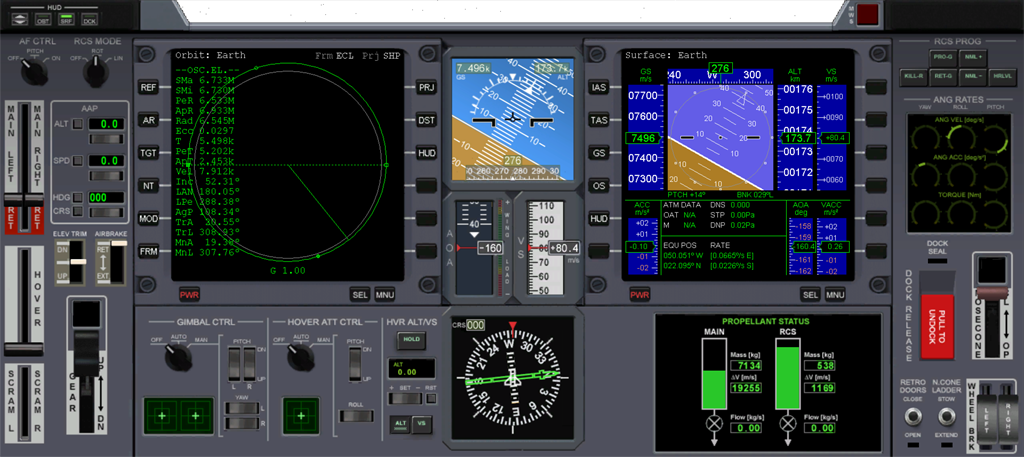
\includegraphics[width=0.99\hsize]{dg_panel_2d.png}
  \caption{Delta-glider main panel}
\end{figure}

\noindent
On opening panel view by cycling the cockpit modes with \keystroke{F8}, you are placed in front of the main panel. Neighbour panels, if present, can be accessed with \Ctrl\DArrow\UArrow\LArrow\RArrow$_{Cur}$. For example, the Delta-glider has an overhead panel that can be called up with \Ctrl\UArrow$_{Cur}$. To return to the main panel, press \Ctrl\DArrow$_{Cur}$.

\begin{figure}[H]
  \centering
  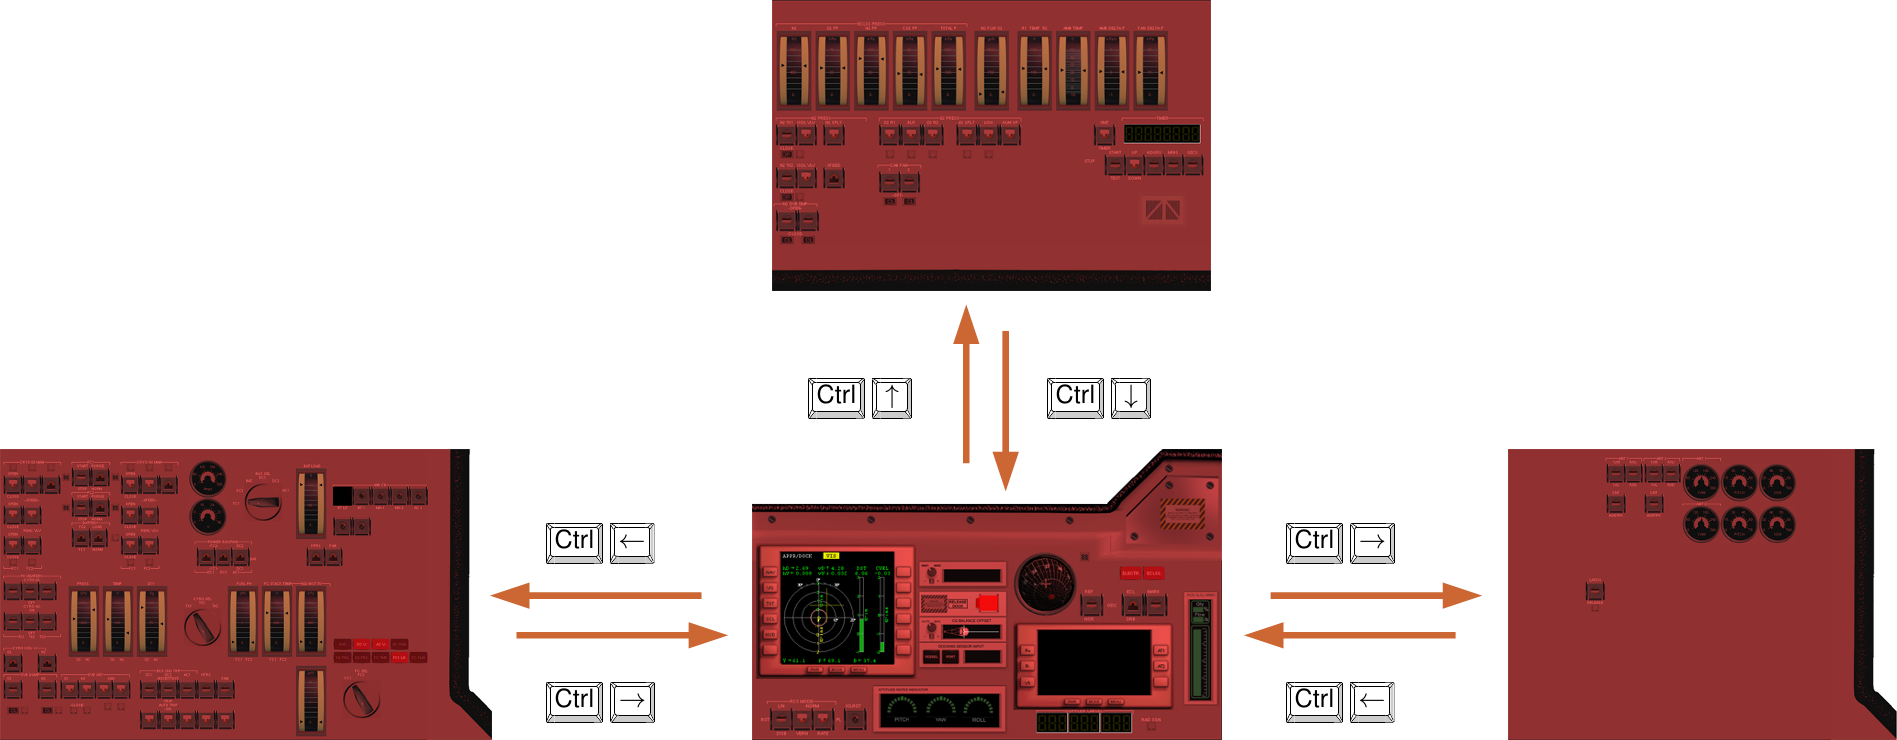
\includegraphics[width=0.99\hsize]{dragonfly_panels.png}
  \caption{Panel connections for the Dragonfly spacecraft.}
\end{figure}

\noindent
Most panels can be scrolled out of the way to get a better view of the surroundings. For example, press \DArrow$_{Cur}$ to scroll the Delta-glider's main panel down. The overhead panel can be scrolled up with \UArrow$_{Cur}$. The scroll speed can be adjusted with the Panel scroll speed option in the \textit{Options} tab of the Orbiter launchpad (see section \ref{ssec:options_tab}).\\
For most vessel types, panels are automatically scaled to fit the simulation window size. If a panel's natural size is larger than the simulation window size and resolution, the panel will be shrunk to fit. In that case, you can zoom into a panel section under the mouse with \Ctrl + mouse wheel.\\
Note that not all vessel implementations may support this feature. Older add-ons use a legacy panel interface which doesn't automatically scale to fit. For such vessels, you can use the Panel scale option in the \textit{Options} tab of the Orbiter launchpad to rescale panels globally (see section \ref{ssec:options_tab}).\\
Panel controls can be operated with the mouse. For details on the panel components of a spacecraft and how to use them, consult the separate documents that come with that vessel.\\
A standard HUD display is superimposed on the panel view. It works the same way as in glass cockpit view. The available HUD modes are described in section \ref{ssec:hud_modes}.\\
The camera view of the outside world can be rotated by right-clicking and dragging the mouse. The field of view can be changed with the mouse wheel. This has no effect on the panel display. The HUD is only visible when looking straight ahead. To return to forward view, press \Home$_{Cur}$.


\subsection{3D virtual cockpit}
The virtual cockpit view places you directly into a 3-D model of the spacecraft cockpit. You can rotate the camera to look around you and access different control panels or get a better view of the outside world (right-click and drag the mouse for rotating the view, or use the coolie hat on your joystick). The mouse wheel zooms the camera in and out and it useful to get a closer look at instruments. Instruments can be operated with the mouse.

\begin{figure}[H]
  \centering
  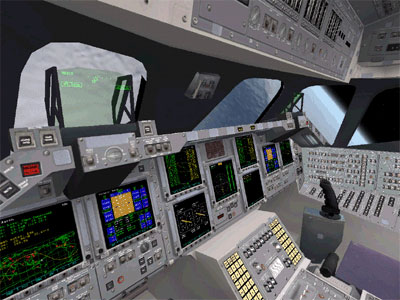
\includegraphics[width=0.99\hsize]{atlantis_vc.jpg}
  \caption{Space Shuttle virtual cockpit}
\end{figure}

\noindent
The virtual cockpit may place a HUD pane in front of the pilot's head. This will then show similar information to the other cockpit views.\\
The pilot position can "lean" in different directions to get a better look out of front or side windows, with \Ctrl\Alt\UArrow\RArrow\LArrow$_{Cur}$. To return to the default position, press \Ctrl\Alt\DArrow$_{Cur}$.\\
The virtual cockpit mode may define multiple operator positions. For example, the Delta-glider allows to switch views from the pilot to the different passenger positions. The Space Shuttle lets you jump from the commander to pilot and payload operator positions. To move between neighbouring positions, press \Ctrl\UArrow\DArrow\RArrow\LArrow$_{Cur}$.

\begin{figure}[H]
  \centering
  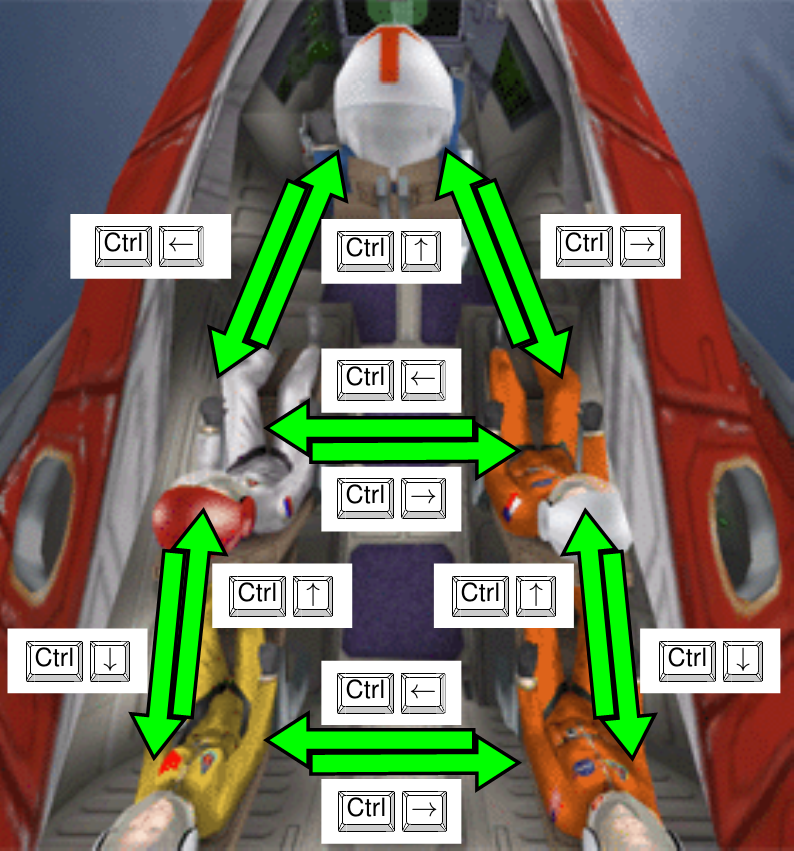
\includegraphics[width=0.5\hsize]{dg_vc_pos.png}
\end{figure}


\subsection{HUD modes}
\label{ssec:hud_modes}
The head-up-display projects flight data into the pilot's line of view without the need to look down at the instruments. In Orbiter, the pilot can set the HUD into different display modes to adjust the projected data to the current flight phase: \textit{surface} (during low-level flight), \textit{orbit} (for orbital manoeuvres) and \textit{docking} (for docking approaches). The HUD mode can be cycled by pressing h. The HUD can be turned on and off with \Ctrl\keystroke{H}.\\
The projection colour can be cycled with \Alt\keystroke{H} to improve display contrast against different backgrounds.\\
All modes display a centre line marker to represent the spacecraft's longitudinal axis (forward direction).\\
\\
\textbf{Surface mode}\\
In \textit{Surface} mode, the HUD provides attitude information relative to the local horizon. At the top, the compass ribbon shows the current heading with regard to true north. If a surface base has been targeted in the Map MFD (see section \ref{ssec:mfd_map}), its bearing is indicated with a marker in the compass ribbon. The pitch ladder shows the current pitch and bank angles. The readout left of the compass ribbon shows true airspeed (TAS) [m/s] if atmospheric density is sufficiently high to measure it, or ground-speed (GS) otherwise. The readout right of the ribbon shows altitude [m] above the mean planet radius (at high altitude) or radar altitude above the surface (at low altitude), indicated by R.\\
The flight path indicator ($\oplus$) represents the current flight direction (the velocity vector in the local horizon frame). A flight path marker located below the centre marker indicates a positive AOA (angle of attack).

\begin{figure}[H]
  \centering
  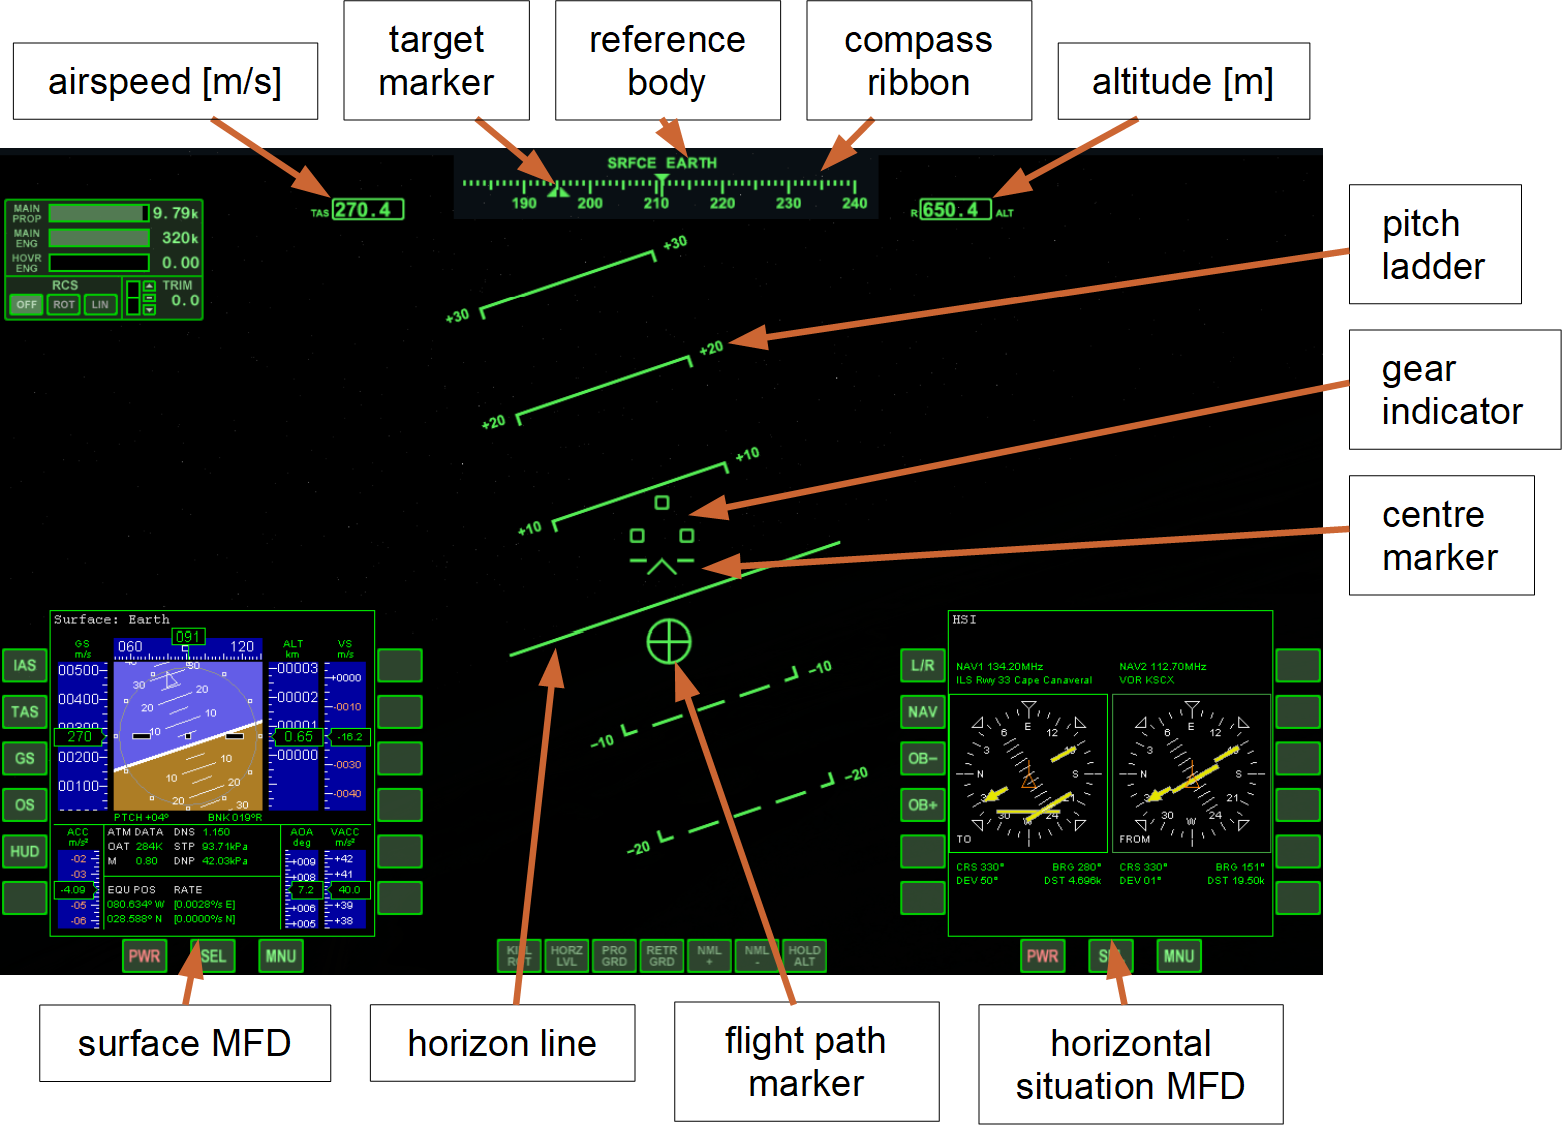
\includegraphics[width=0.75\hsize]{hud_surf.png}
  \caption{Surface HUD elements and relevant MFD modes}
\end{figure}

\noindent
\\
\textbf{Orbit mode}\\
\textit{Orbit} mode is indicated by Orbit \textit{Ref} at the top of the screen, where \textit{Ref} is the name of the reference body being orbited. Orbiter by default selects the main gravitational source as the reference body. This can be manually adjusted with \Ctrl\keystroke{R}, or by selecting a reference body in the \textit{Orbit} MFD (see section \ref{ssec:mfd_orbit}), and pressing the HUD button to copy the choice to the HUD display.\\
The HUD displays a pitch ladder displaying the bank and pitch angles of the spacecraft relative to the orbital plane, where the 0° line represents the orbital plane. A direction ribbon across the centre of the HUD indicates the vessel's yaw deviation from the orbital prograde direction, where 0° and 180° are the prograde and retrograde directions, respectively.\\
The flight path marker ($\oplus$) in Orbit mode represents the orbital velocity vector in the non-rotating reference body frame, i.e. the prograde direction. The retrograde direction is indicated with another marker ($\odot$). If neither the prograde or retrograde direction are within view of the HUD area, the direction of the $\oplus$ marker is indicated with a pointer labelled PG (prograde).

\begin{figure}[H]
  \centering
  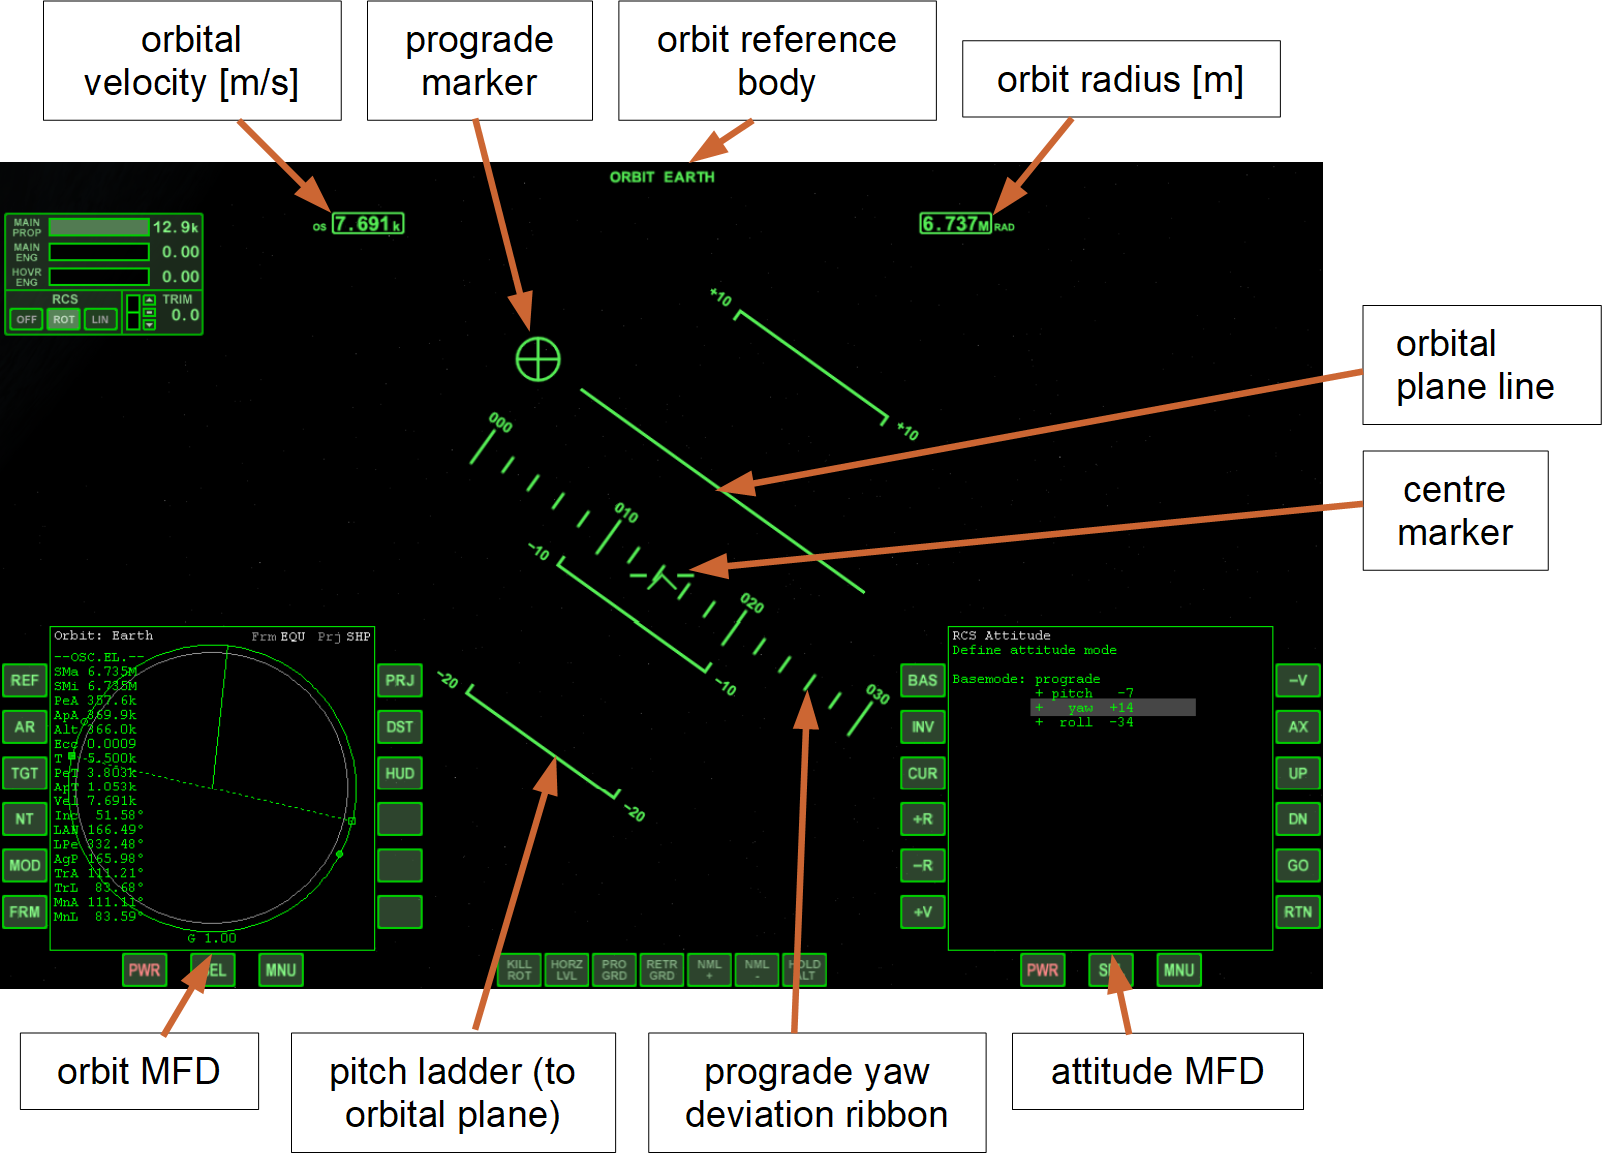
\includegraphics[width=0.75\hsize]{hud_orb.png}
  \caption{Orbit HUD elements and relevant MFD modes}
\end{figure}

\noindent
\\
\textbf{Docking mode}\\
The \textit{Docking} HUD mode assists in approaching and docking with an orbital target, such as a space station. To allow it to display its visual cues it requires target position and velocity data. These are obtained by tuning one of the vessel's NAV radio receivers to either a long-range transponder signal (XPDR) or short-range instrument docking system (IDS) frequencies of one of the target's docking ports. See section \ref{ssec:menu_info} on how to find target transmitter frequencies. See section \ref{ssec:mfd_comnav} on tuning NAV frequencies. Once the NAV receiver has been tuned and is within range of the transmitter, the \textit{Docking} HUD can make use of the target data. Use \Ctrl\keystroke{R} to cycle through the NAV receiver stack. Alternatively, you can pick a receiver in the \textit{Docking} MFD mode and copy it to the HUD by pressing the HUD button. NAV and target signal designations are shown in the top of the HUD area.\\
Alternatively, you can bypass the NAV receiver data acquisition and target an object or docking port directly by pressing \Ctrl\Alt\keystroke{R}. If you are close to a docking port, you can also press the VIS button on the Docking MFD for visual docking approach acquisition, followed by HUD to copy the data to the HUD display.\\
The position of the target object is marked with a square box, labelled with the object name and distance [m]. If the target object is not visible in the area covered by the HUD, its direction is indicated with a pointer.\\
The vessel's velocity vector relative to the target object is indicated with the flight path indicator ($\oplus$). It is labelled with the magnitude of the relative velocity [m/s]. The opposite direction (or the velocity vector of the target relative to your ship) is indicated with $\odot$ and a negative velocity label. If neither velocity marker is visible in the HUD, the direction of the $\oplus$ marker is indicated with a pointer.\\
If the HUD display is bound to a receiver tuned to an IDS signal, the approach path to the dock is symbolised with a series of virtual approach gates. These are rectangles spread along the approach path. The "up" direction (for bank alignment) is indicated with a double line.

\begin{figure}[H]
  \centering
  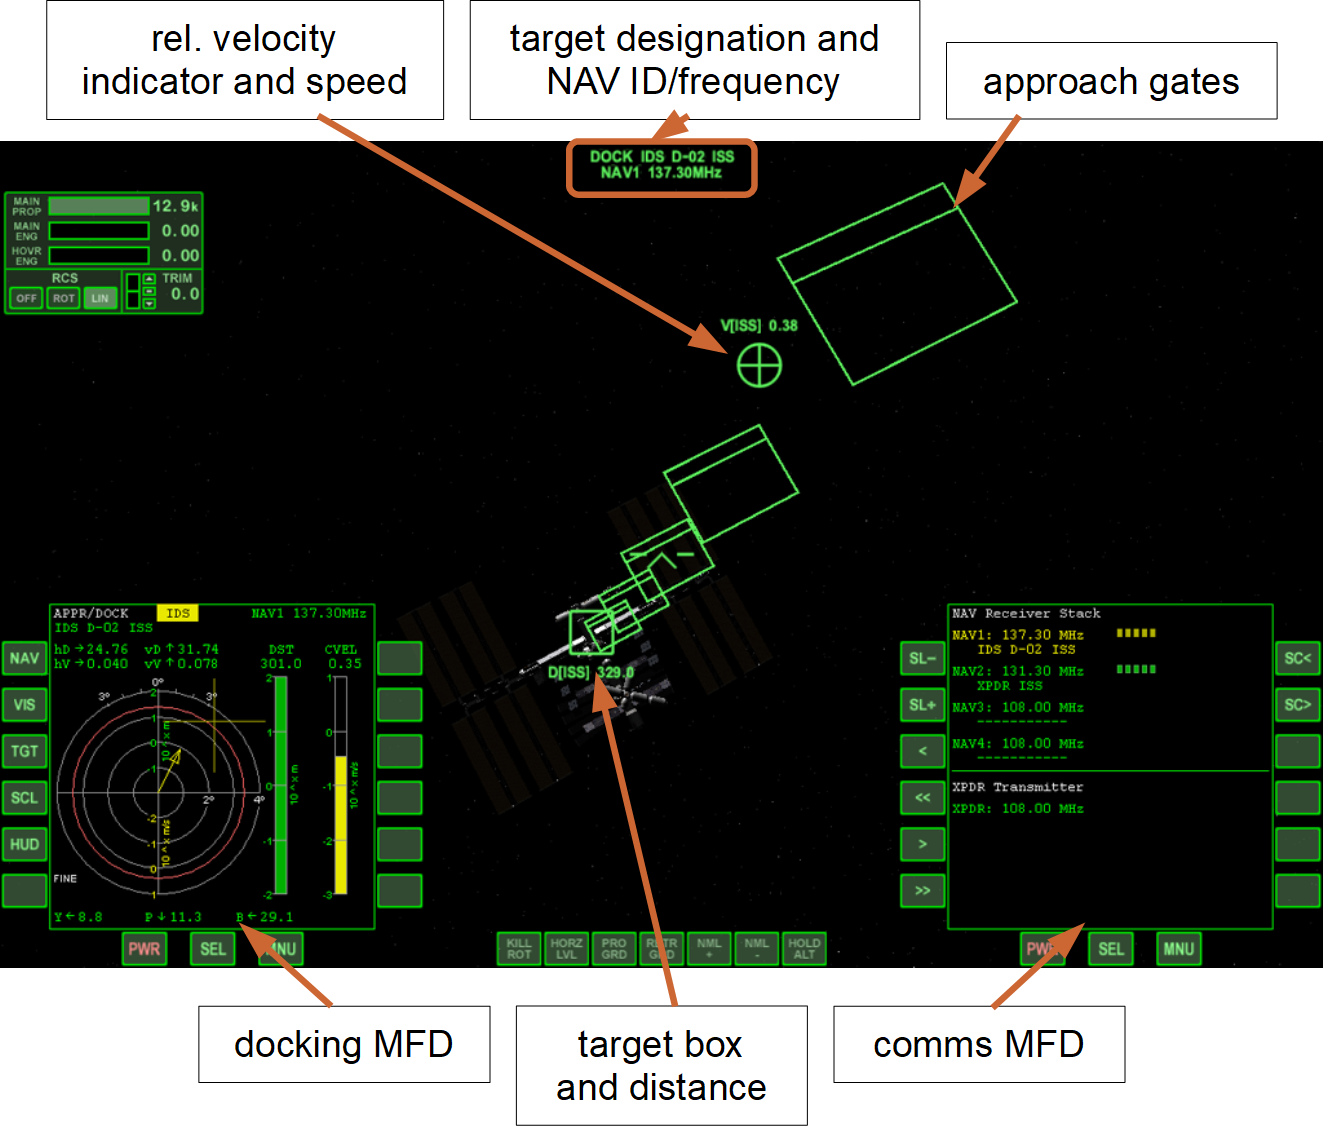
\includegraphics[width=0.75\hsize]{hud_dock.png}
  \caption{Docking HUD elements and relevant MFD modes}
\end{figure}


\end{document}
